\chapter{质谱}
\begin{introduction}
    \item 质谱峰基本知识(熟悉)
    \item 质谱仪结构(熟悉)
    \item 质谱定量分析(了解)
    \item 质谱谱图解析(了解)
\end{introduction}
\section{质谱}
\begin{definition*}{质谱}
    利用离子化技术,将物质分子转化为离子,按照其质荷比(m/z)的大小依次排列构成质谱。并利用质谱进行定性、定量和结构分析的方法。
\end{definition*}
质谱的特点:
\begin{itemize}
    \item (1)进样量少、灵敏度高、分析速度快
    \item (2)唯一可以给出分子量,确定分子式的方法
\end{itemize}


\section{质谱仪}

基本构造:进样系统$\rightarrow$离子源$\rightarrow$质量分析器$\rightarrow$检测器$\rightarrow$真空系统

原理:分子在气态、液态或固态被电离,离子在高压电场中加速,在磁场中偏转到达收集器,产生信号。强度与到达的离子数目成正比。

质谱仪的种类:
\begin{itemize}
    \item 有机质谱仪:气相/液相色谱-质谱联用仪、基质辅助激光解析电离飞行时间质谱仪、傅里叶变换质谱仪
    \item 无机质谱仪:电感耦合等离子体质谱仪、火花源双聚焦质谱仪、二次离子电离质谱仪
    \item 同位素质谱仪:小型低分辨率同位素质谱仪(轻元素——H,C,S)、大型同位素质谱仪(重元素——U,Pu,Pb)
    \item 气体分析质谱仪:呼气质谱仪、氦质谱检漏仪
\end{itemize}
\subsection{电离源/离子源}
\begin{itemize}
    \item 气相源:先蒸发再激发,适于沸点低于500℃、对热稳定的样品的离子化,包括电子轰击源、化学电离源、场电离源、火花源。
    \item 解吸源:固态或液态样品不需要挥发而直接被转化为气相,适用于分子量高达105的非挥发性或热不稳定性样品的离子化。包括场解吸源、快原子轰击源、激光解吸源、离子喷雾源和大气压化学(热喷雾)电离源等。
    \item 硬源:离子化能量高,伴有化学键的断裂,谱图复杂,可得到分子官能团的信息,如电子轰击,快原子轰击。
    \item 软源:离子化能量低,产生的碎片少,谱图简单,可得到分子量信息,如化学电离源,场电离源,场解吸电离源,激光解吸电离源,电喷雾电离源,大气压化学(热喷雾)电离源。
\end{itemize}
电子源的类型
\begin{itemize}
    \item 电子电离源(EI)
    
    特点:工作稳定可靠,结构信息丰富,有标准质谱图。但只适用易汽化的有机物样品分析,并且有些化合物得不到分子离子峰。

    适用范围:主要适用于易挥发性有机样品的电离

    原理:在热丝阴极与阳极之间加上电压,热阴极发射出高能电子束,在高速向阳极运动时,撞击来自进样系统的样品分子,使样品分子发生电离。

    \begin{note}
        形成离子的途径:分子被打掉一个电子形成分子离子、分子离子化学键断裂形成碎片离子、分子离子结构重排形成重排离子、分子离子反应生成加合离子
    \end{note}
    \item 化学电离源(CI)
    
    特点:\begin{itemize}
        \item 准分子离子峰即(M+1)+峰很强,可提供相对分子质量
        \item 软电离源,碎片峰较少,谱图简单,因为电离样品分子的不是高能电子流,而是能量较低的二次离子,键断裂的可能性较小 
        \item  用CI时需要将试样气化后进入离子源,因此不适用于难挥发,热不稳定或极性较大的有机物分析。对于不稳定的有机化合物,可得到较强的分子离子峰
        \item 不是标准质谱,所以不能进行库检索
    \end{itemize}

    适用范围:适用于易汽化的有机样品分析品的离子化

    原理:高能量的电子轰击反应气体使之电离,电离后的反应分子再与试样分子碰撞发生分子离子反应形成准分子离子和少数碎片离子。
    \begin{example}
    以CH4稀释时,出现$(M+1)^{+}$,$(M-1)^{+}$,$(M+17)^{+}$,$(M+29)^{+}$等质谱峰
    \end{example}
    \begin{note}
        EI 和 CI 主要用于气相色谱-质谱联用
    \end{note}
    \item 快原子轰击(FAB)
    
    特点:
    \begin{itemize}
        \item 属于二次离子质谱,使用中性原子束作为初级高能量粒子轰击表面,再对由此产生的二次离子进行质谱分析。
        \item 以液体基质负载样品,实验时通常预先将试样和底物调和并涂在金属靶上。
        \item 理想的基质必须蒸汽压低,对试样的质谱干扰小,同时是被分析样品的良好溶剂(常用的有甘油、硫代甘油、三乙醇胺等)
        \item 质谱的分子量信息不是分子离子峰M,而往往是(M+H)+或(M+Na)+等准分子离子峰;谱图碎片少
        \item 会出现基质分子产生的相应的峰及基质分子与样品分子的结合峰
    \end{itemize}

    适用范围:适用于难气化, 极性强的大分子,如肽类、低聚糖、天然抗生素、有机金属配合物

    原理:惰性气体Ar或Xe的原子依靠放电首先被电离并被加速,使之具有高的动能,在原子枪(atom gun)内进行电荷交换反应:
   \begin{equation*}
    Ar^{+}_{\text{高动能}}+ Ar_{\text{热运动}}\rightarrow Ar_{\text{高动能}}+ Ar^{+}_{\text{热运动}}
   \end{equation*} 
    高动能的Ar或Xe原子束再轰击样品分子使其离子化
    
    \item 场致电离源(FI)
   
    特点:
    \begin{itemize}
        \item 场致电离源的能量约为12eV,因此分子离子峰强度很大,也很清楚,碎片峰较少也较弱,利于相对分子质量的测定,缺乏分子结构信息
        \item 电极为一尖锐的叶片或金属丝,其上长满微针,故称金属胡须发射器。
        \item 使用微碳针构成多尖阵列电极可提高电离效率
    \end{itemize}

    原理:应用强电场诱导样品电离。
    强电场$\rightarrow$分子电子的量子隧道效应* $\rightarrow$分子热分解或碰撞$\rightarrow$带正电荷的碎片离子$\rightarrow$阳极排斥出并加速进入质量分析器

    \item 场解析电离源(FD)
   
    特点:
    \begin{itemize}
        \item 谱图最为简单(解吸所需的能量远低于气化所需的能量,所以有机化合物不会发生热分解)
        \item 离子源的工作温度略高于室温,分子离子几乎不具有过剩的能量,因此基本上不断裂,分子离子峰的强度比FI强
    \end{itemize}

    适用范围:非挥发性且分子量高的样品

    原理:样品溶液涂于发射器表面$\rightarrow$通电加热蒸发除溶剂$\rightarrow$解吸样品分子$\rightarrow$强电场$\rightarrow$分子电离$\rightarrow$奔向阴极$\rightarrow$引入质量分析器

    \item 电喷雾电离(ESI)
    
    特点:
    \begin{itemize}
        \item 主要应用于LC-MS(液相色谱-质谱联用),既是接口装置,又是电离源
        \item 即使分子量大,稳定性差的化合物,也不会在电离过程发生分解
        \item 产生的离子带有多电荷
        \item 两层套管组成的电喷雾喷嘴,内层是LC流出物,外层是雾化气,喷嘴上加3-5kV正电压,与相距约1cm接地的反电极形成强静电场
    \end{itemize}

    适用范围:适用于强极性,大分子量的样品分析如肽,蛋白质,糖等

    原理:被分析的样品溶液从毛细管流出时在电场作用下形成高度荷电的雾状小液滴;喷嘴前方的补助气喷嘴使小液滴进一步雾化,加速溶剂蒸发,阻止中性的溶剂分子进入质量分析器。
    液滴因溶剂的挥发逐渐缩小,其表面上的电荷密度不断增大。当电荷之间的排斥力足以克服表面张力时,液滴发生裂分;经过反复的溶剂挥发-液滴裂分过程,最后产生单个多电荷离子。

    \item   大气压化学电离源 (APCI) 
    
    \textcolor{blue}{大致类似ESI}

    共同点:
    \begin{itemize}
        \item 使用高电压元件和雾化气喷雾法产生离子
        \item 通常产生$(M+H)^{+}$或$(M-H)^{-}$等准分子离子
        \item 产生极少的碎片,可以控制产生结构碎片
        \item 非常灵敏的电离技术
    \end{itemize}

    不同点:
    \begin{itemize}
        \item 生成离子的方式不同
        \begin{itemize}
            \item ESI:液相离子化
            \item APCI:气相离子化
        \end{itemize}
        \item 样品兼容性不同
        \begin{itemize}
            \item ESI:极性化合物和生物大分子
            \item APCI:非极性,小分子.化合物(相对ESI而言)且有一定挥发性 
        \end{itemize}
        \item 流速兼容性
        \begin{itemize}
            \item ESI:0.001到1 mL/min
            \item APCI:0.2到2mL/min 
        \end{itemize}
        \item ESI的适用范围要远远大于APCI
        
        ACPI适用中等极性(小于1000 Da)的化合物,产生单电荷离子

        与ESI大致相同,不同之处在于APCI喷嘴的下游放置一个针状放电电极,通过它的高压放电,使空气中某些中性分子电离,产生\ce{H3O+},\ce{N2+}和\ce{O2-}等离子,溶剂分子也会被电离,这些离子与分析物分子进行离子-分子反应,使分析物分子离子化
    \end{itemize}
    \item 基质辅助激光解析电离(MALDI)
    
    特点:得到分子离子峰,无明显碎片峰。 此电离方式特别适合于飞行时间质谱计。
    \begin{note}
        常用的基质有:2,5-二羟基苯甲酸、芥子酸、烟酸、$\alpha$-氰基-4-羟基肉桂酸
    \end{note}

    适用范围:MALDI适用于生物大分子,如肽类、蛋白质和核酸类化合物。

    原理:待测物质与基质的溶液混合后蒸发,使分析物与基质成为晶体或半晶体,利用一定波长的脉冲式激光照射样品激光照射到样品靶上,基质分子吸收并传递激光能量,与样品分子一起蒸发到气相,并使样品分子电离

    \item 电感耦合等离子体(ICP)
    
    原理:高频电流通过感应线圈产生变化的高频磁场,此时向矩管的外管内切线方向通入Ar,中层管内轴向通入辅助气体Ar,并用高频点火装置引燃,产生载流子(离子或电子)。 电子密度增加,达到足够的导电率时,就会产生异构垂直于管轴方向的环形涡电离,迅速将载气加热到几千乃至上万度,并在石英管口形成等离子炬。样品气溶胶瞬间在等离子体中被解离,形成被电离的分析原子。
\end{itemize}

\subsection{质量分析器}
将离子源中形成的不同离子按质荷比(m/z)的大小分开,将质荷比相同的离子聚集在一起。主要为磁分析器:

原理:主要部分是一对电磁铁(常用扇形),当离子源中产生的离子束经加速电场加速后,以一定的速度进入垂直于离子运动方向的均匀磁场时,离子在磁场施加的向
心力的作用下,改变运动方向(磁场不改变离子的运动速度)作圆周运动,运动轨道半径与运动速度、磁场强度、离子的质荷比有关
公式:
\begin{theorem*}{磁分析器原理}
    \begin{equation*}
        \frac{m}{z}=\frac{H^{2}R^{2}}{2U}
    \end{equation*}
\end{theorem*}

测试时,固定H、R、U中任意两个,连续改变另一个,即得质谱图。现代质谱仪通常固定R,改变U或H来得到质谱图。
\subsubsection*{单聚焦质量分析器}
磁场是扇性磁场,扇性开角是180或90°。只能实现方向聚焦。无法实现能量聚焦,故其分辨率较低,一般为500,只能用于同位素和气体质谱。
\subsubsection*{双聚焦质量分析器}
在扇形磁场前加一同轴扇形电极组成的静电场(场强E),离子做半径为$R_{e}=\frac{2U}{E_{e}}$
的圆周运动,对于动能不同的离子,通过调节电场能,达到聚焦的目的。

特点:同时具有方向聚焦和能量聚焦, 高分辨率(十几万甚至上百万)但是体积较大
\subsubsection*{四级杆分析器}
四根截面为双曲面或圆形的平行杆组成,对角的电极为一组,在两个相对的极杆之间加电压$U+Vcos\omega t$(U 为直流电压,$Vcos\omega t$是射频电压),在另两个相对极杆间加$-(U+Vcos\omega t)$高速运动的离子束穿过准直小孔进入四极杆之间的空间时,在高频电场的作用下发生振荡,在一定的电压和频率下,只有一种质荷比的离子会形成稳定的振荡通过四极杆到达检测器,其余离子则因振幅不断增大,撞在电极上而被真空泵抽出。 使交流电压的频率不变,连续的改变直流和交流电压的大小(保持他们的比例不变)(电压扫描)或保持电压不变连续的改变交流电压的频率(频率扫描),就可使不同质荷比的离子依次到达检测器。

特点:分辨率比磁分析器略低(max.2000); m/z范围与磁分析器相当;传输效率较高;扫描速度快,可用于GC-MS 联用仪

\subsubsection*{飞行时间质量分析器}
离子漂移管加速后的离子具有相同的动能。m/z小的离子,漂移运动的速度快,最先通过漂移管,到达检测器;m/z大的离子,漂移运动的速度慢,最后通过漂移管,到达检测器。检测通过漂移管的时间( t )及其相应的信号强度。
适合于生物大分子,灵敏度高,扫描速度快,结构简单,分辨率随m/z的增大而降低。

线性飞行时间质谱分辨率较低的改进方法: 
\begin{itemize}
    \item  引进反射器:两个质量相同,初始动能不同的离子,动能大的在反射器内飞行时间较长,动能小的在反射器内飞行时间较短。因此在反射器的作用下,飞行时间得以补偿,最终使得这两个离子几乎同时到达检测器。
    \item 延迟引出:样品分子电离后延迟再加速,可以补偿离子初始动能分布对分辨率的影响。
\end{itemize}

特点:
\begin{itemize}
    \item 仪器结构简单,操作容易,不需要磁场、电场等
    \item 无聚焦狭缝,灵敏度很高
    \item 可用于大分子的分析(几十万原子量单位)
    \item 扫描速度快(1000幅/s),可用于研究快速反应或与GC联用
    \item 分辨率比磁分析器稍差,受飞行距离的限制
\end{itemize}

\subsubsection*{离子阱质量分析器}
上下端罩电极与左右环电极构成可变电场形成阱,当直流电压和射频电压一定时,只有特定m/z的离子能在阱中指定的轨道上稳定旋转,并可长时间留在阱内,其它离子将偏出轨道并与环电极发生碰撞而消失。
特点:结构简单、易于操作、GC-MS联用可用于m/z200-2000 的分子分析。

\begin{definition*}{MALDI-TOF-MS:}
    基质辅助激光解析电离飞行时间质谱,是一种软电离技术(详细内容见上表)。适用于混合物及生物大分子的测定,如肽类、蛋白质和核酸类化合物。
\end{definition*}

\section{质谱谱图解析}
\subsection{基本要素}
\begin{definition*}{分子离子峰}
    在电子轰击下,分子失去一个电子所形成的离子叫分子离子,所出的峰便是分子离子峰
\end{definition*}
\begin{note}
    标记方式:奇电子离子(OE)标为“+·”,偶电子离子(EE)标为“+”。若分子含杂原子,则电荷标在杂原子上;若不含杂原子而含双键,则标在双键的一个碳上;若既无杂原子又无双键,则标在分支碳原子上;若位置不确定则在右上角标“┐+”。
\end{note}

作用
\begin{itemize}
    \item 获得相对分子量
    \item 根据分子离子和相邻荷质比较小碎片离子的关系,可判断化合物类型及可能含有的官能团
    \item 由分子离子及同位素峰的相对强度,可推导分子式
\end{itemize}

\begin{note}
    辨认分子离子峰的方法
    \begin{itemize}
        \item 各类有机物分子离子峰稳定性顺序:芳香化合物>共轭链烯>烯烃>脂环化合物>直链烷烃>酮>胺>脂>醚>酸>支链烷烃>醇
        \item N律:由C、H、O组成的有机物,M一定为偶数;含C、H、O和偶数个N的化合物,M一定为偶数;含C、H、O和奇数个N的化合物,M一定为奇数
        \item 分子离子峰与相邻峰质量差必须合理,若质量差为3~14,19~25等,则最高质量峰不是分子离子峰
        \item 可通过降低电子轰击源的电压,采用软电离或把不稳定样品制成适当衍生物的方法增强分子离子峰
    \end{itemize}
\end{note}
 \begin{definition*}{同位素离子峰}
    由于同位素的存在,可以看到比分子离子峰大一个质量单位的峰;有时还可以观察到M+2,M+3
 \end{definition*}
 \begin{definition*}{ 碎片离子峰}
   一般有机化合物的电离能为7-13 eV ,质谱中常用的电离电压为70 eV,使结构裂解,产生各种“碎片”离子
 \end{definition*}
 \begin{definition*}{亚稳离子峰}
    离子在离开离子源被加速过程中或在加速之后进入质量分析器之前在无场区内发生裂解而形成的离子所产生的峰,称为亚稳离子峰。可用于寻找裂解途径。特点:峰弱,峰钝,质荷比一般不是整数
 \end{definition*}
\begin{theorem*}{麦氏重排}
    要求:含有C=O, C=N,C=S及C=C。与双键相连的链上有γ碳,并在γ碳上有H原子(γ氢)。
六元环过渡,γ-H转移到杂原子上,同时β键发生断裂,生成一个中性分子和一个自由基阳离子。

\end{theorem*}
\begin{figure}[ht]
    \centering
    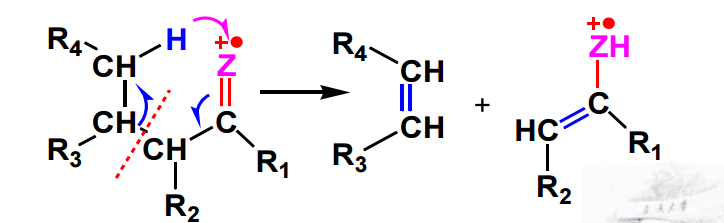
\includegraphics[width=5cm]{image/chp2_m_reform.png}
    \label{fig:chp2_reform}
    \caption[]{麦氏重排}
\end{figure}



\subsection{质谱定性定量分析}
\subsubsection*{烃类}
\begin{itemize}
    \item 直链烷烃
    
    直链烷烃分子离子峰强度不高,强度随碳链增长而降低,通常碳数<40的烷烃分子离子峰(M+. )尚可观察到。
    有相差14个质量数的一系列奇质量数的峰($C_{n}H_{2n+1}$ )强度逐渐减弱, m/z 43和m/z 57的峰强度较大。
    在比$C_{n}H_{2n+1}$ 离子小一个质量数处有一个小峰,即$C_{n}H_{2n}$ 离子峰,其一系列弱峰是由H转移重排成的.
    系列$C_{n}H_{2n-1}$ 的碎片峰,由 $C_{n}H_{2n+1}$ 脱去一个H2中性分子。
    \item 支链烷烃
    
    分子离子峰的强度比正构烷烃的弱,支链越多分子离子峰( $M^{+\cdot}$ )强度越弱。
    在分支处容易断裂,正电荷在支链多的一侧,丢失最大烃基为最稳定。在质谱图中若有M-15峰,则表明结构中存在甲基支链。
    \item 烯烃
    
    分子离子峰较强;
    单烯的σ断裂得到一系列m/z相差14的$C_{n}H_{2n-1}$ 碎片离子峰;
    易发生β开裂,生成m/z 41的烯丙基正碳离子$C_{3}H_{5}^{+}$。
    \item 芳烃
    
    分子离子稳定,有较强的分子离子峰;
    烷基取代苯易发生$\beta$裂解,经重排产生m/z 91特征的卓鎓离子,很稳定常为基峰。
    卓鎓离子可进一步裂解生成m/z 65的环戊二烯、m/z 39的环丙烯正离子。
    取代苯可发生$\alpha$裂解,产生m/z 77的苯离子,进一步裂解生成环丙稀离子及m/z 51的环丁烯离子。
    具有$\gamma$氢的烷基取代基,可发生麦氏重排裂解,产生m/z92($C_{7}H_{8}$)重排离子。
\end{itemize}

\subsubsection*{ 羟基化合物}
\begin{itemize}
    \item 脂肪醇

    分子离子峰很弱,随碳链增长减弱至消失,长链醇可发生$\alpha-,\beta-,\gamma-,\delta-$裂解。
    $\alpha-$断裂是醇类的主要裂解,质谱图中的主要碎片几乎都是α-断裂产生的,生成一组鐊鎓离子。易发生脱水重排反应,产生M-18离子
    \item 酚和芳香醇
    
    分子离子峰很强,酚的M+往往是基峰。
酚类和苄醇类最具有特征的峰是失去CO和CHO所形成M-28和M-29。
\end{itemize}

\subsubsection*{醚的质谱图}
\begin{itemize}
    \item 脂肪醚
    
    脂肪醚的分子离子不稳定是弱峰,主要裂解方式是$\alpha -$断裂,生成较强的m/z45、59、73、87……的峰。
    i-断裂时C—O键断裂产生OR自由基及烷基正离子
    \item 芳醚
    
    芳醚的分子离子峰较强;苯甲醚的β-裂解形成m/z 93 碎片很容易脱去CO产生稳定的m/z 65的离子(出现相应的亚稳离子)
\end{itemize}
\subsubsection*{羰基的质谱图}
\begin{itemize}
    \item  醛
    
    脂肪醛的分子离子峰较明显,大于C4的脂肪醛分子离子峰强度明显递减。
    
    芳香醛的分子离子峰更稳定。
    易发生$\alpha$裂解,产生$R^{+}(Ar^{+})$、m/z 29及M-1离子峰。
    具有$\gamma$氢的醛,能发生麦氏重排,产生m/z 44的乙烯醇
    如果$\alpha$位有取代基,还会出现m/z (44+14n)重排离子。
    长链脂醛还可发生$\beta$裂解,生成无氧碎片系列离子峰m/z 29, 43, 57…(29+14n)
    \item  酮
    
    脂肪酮的分子离子峰很强,但随分子量的增加而减弱。易发生$\alpha$裂解,具有$\gamma$氢的酮也能发生麦氏重排。
    \item 酸和酯
    
    一元饱和羧酸及其酯的分子离子峰较弱,芳酸与其酯的则较强。
    易发生$\alpha$裂解,具有$\gamma$氢的羧酸与酯易发生麦氏重排。
\end{itemize}

\subsection{简单的质谱解析及其应用}
\begin{note}
    

\textcolor{red}{谱图解析的一般方法:}
\begin{itemize}
    \item(1) 由高质量端求出分子离子峰,初步判断有无Cl、Br、S等元素;
    \item(2) 根据分子离子峰的高分辨数据给出化合物组成式;
    \item(3) 由组成式计算不饱和度;
    \item(4) 研究高质量端离子峰,由于它们是分子离子失去碎片形成的,从失去碎片可以确定取代基;
    \item(5) 研究低质量端离子峰,寻找不同化合物的特征离子和特征离子系列(见上一部分),推测化合物类型;
    \item(6) 提出可能结果,必要时通过红外或核磁进一步确定;
    \item(7) 验证所得结果。
\end{itemize}
\end{note}

\section*{补充:常用色谱仪种类}
\subsection*{气相色谱-质谱联用仪(GC-MS)}
质谱仪是一种很好的定性鉴定用仪器,但对混合物的分析无能为力;色谱仪是一种很好的分离用仪器,但定性能力差。

GC-MS由3部分组成:色谱部分、质谱部分、数据处理系统。色谱部分和一般色谱仪基本相同,混合样品在合适的色谱条件下被分离成单个组分进入质谱部分进行鉴定。质谱部分在高真空下工作,因此如果色谱仪使用填充柱必须使用经过一种接口——分子分离器,将色谱载气去除;色谱仪使用毛细管柱,可以将毛细管直接插入质谱仪离子源。质谱部分最常用四极质谱仪,离子源主要是EI源和CI源。

GC-MS要求样品最好是液态,固态样品必须溶解。GC-MS分析得到的主要信息有个:总离子色谱图、每一个组分的质谱图、每个质谱图的检索结果。
\subsection*{液相色谱-质谱联用仪(LC-MS)}
对于热稳定性差或不易汽化的样品,GC-MS存在一定困难,需改用LC-MS分析,特别是生物大分子的分析。LC-MS联用的关键是LC和MS之间的接口装置,主要作用是去除溶剂并使样品离子化。

目前几乎所有的LC-MS都是用大气压电离源作为接口装置和离子源,大气压电离源包括电喷雾电离源(ESI)和大气压化学电离源(APCI)。LC-MS得到的信息与GC-MS类似。由于ESI只产生准分子离子,因此质谱图较为简单,质谱采集时刻采正离子、负离子或同时采集正、负离子。这种质谱过于简单,为克服这一缺点,在LC-MS中MS部分最好采用串联质谱仪。
\subsection*{ 基质辅助激光解析电离飞行时间质谱仪(MALDI-TPF)}
  样品放置在可以移动的靶板上,依靠激光将样品电离,并由飞行时间质谱仪得到质谱。主要特点是质量范围宽,分辨率高,利用源后裂解技术(PSD)可以得到结构信息。主要用于生物大分子的分析。